\subsection{Profile Screens}\label{subsec:profile-screens}
The \textbf{Profile screen} (Figure~\ref{fig:profile}) represents the main menu of the application.
Users have granted access to their profile detail, My management container, and the users can see the set default aircraft and device.
Besides, if they belong to an organization, it shows them the organization name and the button to switch the fleet mode.
My management container contains My Flights, My Devices and My Aircrafts buttons.

The \textbf{Profile detail} screen contains the user properties like the full name, phone number and country.
Also, it allows changing the user's contact e-mail and password.


\begin{figure}
    \centering
    \begin{minipage}{.4\textwidth}
        \centering
        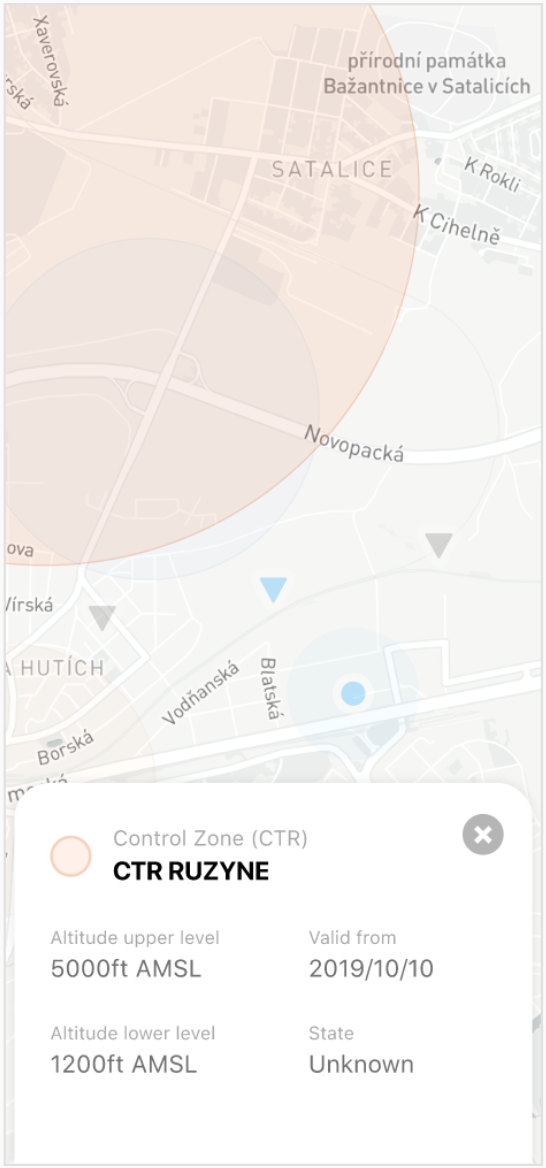
\includegraphics[width=.7\linewidth]{assets/user_interface_design/dashboard/dashboard_zone_detail.png}
        \caption{Dashboard, Zone detail}
        \label{fig:dashboard_zone_detail}
    \end{minipage}%
    \hspace{.05\linewidth}
    \begin{minipage}{.4\textwidth}
        \centering
        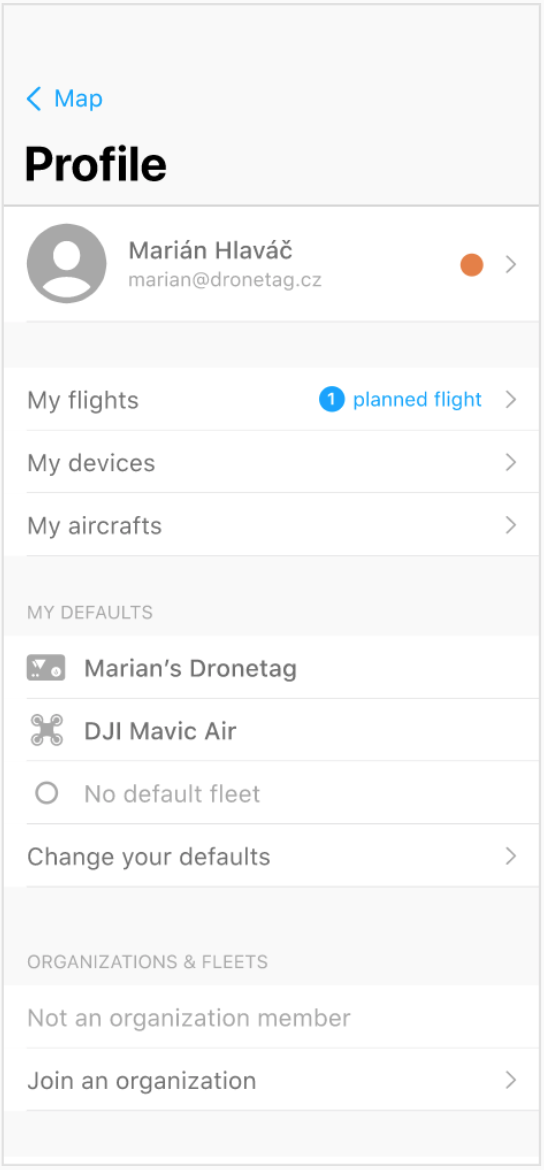
\includegraphics[width=.7\linewidth]{assets/user_interface_design/profile/profile.png}
        \caption{Profile}
        \label{fig:profile}
    \end{minipage}
    \label{fig:profile_all}
\end{figure}
